%!TEX root = Manuscript.tex

\chapter{Proof of feasibility}
\label{chap:TSN}
\minitoc
The main objective of this thesis is to achieve the lowest possible latency. To do so, it is necessary that packets are not delayed in the network. Delay causes are various, but the main one if the buffering time. In store-and-forward concept~\cite{tindell1992store}, packets are stored at reception of a node before to be forwarded. However, solution like cut-through~\cite{kermani1979virtual} allow to reduce storage size and corresponding delay to the header size only. But this is effective if the egress port is available to forward the packet at the same time only. If not, the packet is buffered until the port get free. This situation needs to be avoided.

This chapter present in Section~\ref{sec:TSNqbv} the IEEE standards for Time Sensitive Networking (TSN) and more precisely 802.1 Qbv, that allows a better network managment based on scheduled packets. 

The platform presented in Section~\ref{sec:platform} goes beyond TSN, by delivering packet at exact expected dates, achieving what we call “Hyper TSN”. In Hyper TSN, the latency is as close as possible with physical limitations.


\section{Link between the model and TSN}

The model we present in Chapter~\ref{chap:model} is based on several assumption. We explain in this chapter how the recent standards developed by TSN task group brings us to such a model.

\todo{ref papier ultime arxiv}


The stadard IEEE 802.1Qat SRP (Stream Rerservation Protocol) provides a central managment framework that allow a centralized entity to collect datas about the flows over the network and to reserve bandwidth for the flows. It has been improved by IEEE 802.1Qcc. Those standards allows us to centralize all required information needed by our algorithm about the network (the routing, the length of the links, the periodicity andthe size of the datagrams) in a centralized entity that we call \bf{controller}. This controller has a user interface that allows us to collect those informations in order to compute the best assignment with the algorithms of previous chapters.


Once the scheduling of the datagram is computed, the switchs needs to be able to forward the packet at the right exact date, differentiating the flows, without any additional latency. This is fully covered by TSN 802.1 Qbv, as explained in [intro]: Rappeler tout qbv + expliquer que ca couvre aussi statistical multiplexing

We consider that the components of the network are completely synchronized. Such an hypothesis seems unrealistic, but standards likes IEEE 802.1ASrev, or IEEE 1588 \todo{refs} propose good solutions for clock synchronization. This issue is fully covered by Hyper-TSN switch of the next section \todo{J'en sais rien en fait?}.


\begin{figure}
\begin{center}
\scalebox{0.4}{

\begin{tikzpicture}
  \SetGraphUnit{5}
    \tikzset{
  EdgeStyle/.append style = {->} }
   \tikzstyle{VertexStyle}=[shape = circle, draw, minimum size = 30pt]
 

  \node (r1) at (0,0) {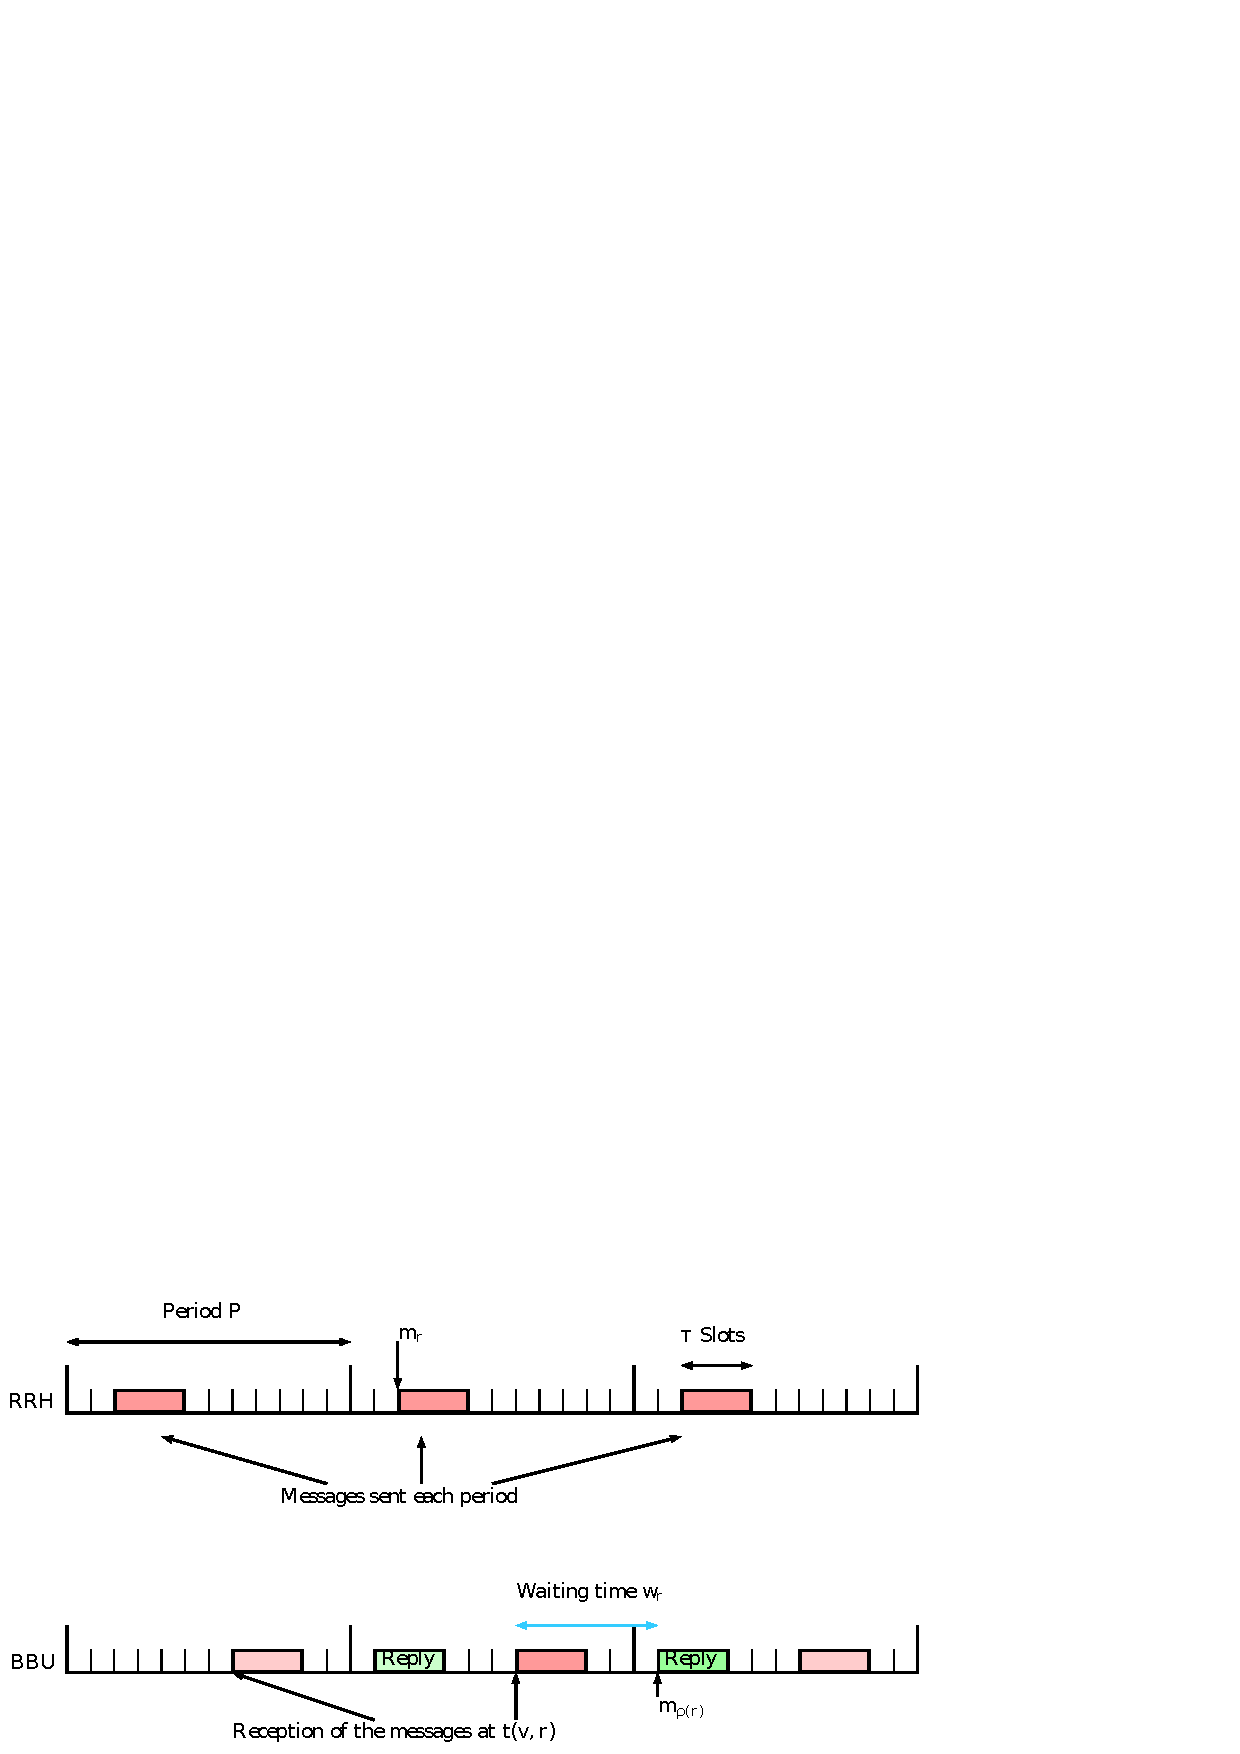
\includegraphics[width = 1cm]{rrh.png}};
   \node[below] at (r1.south) {RRH};
  \node (r2) at (0,4) {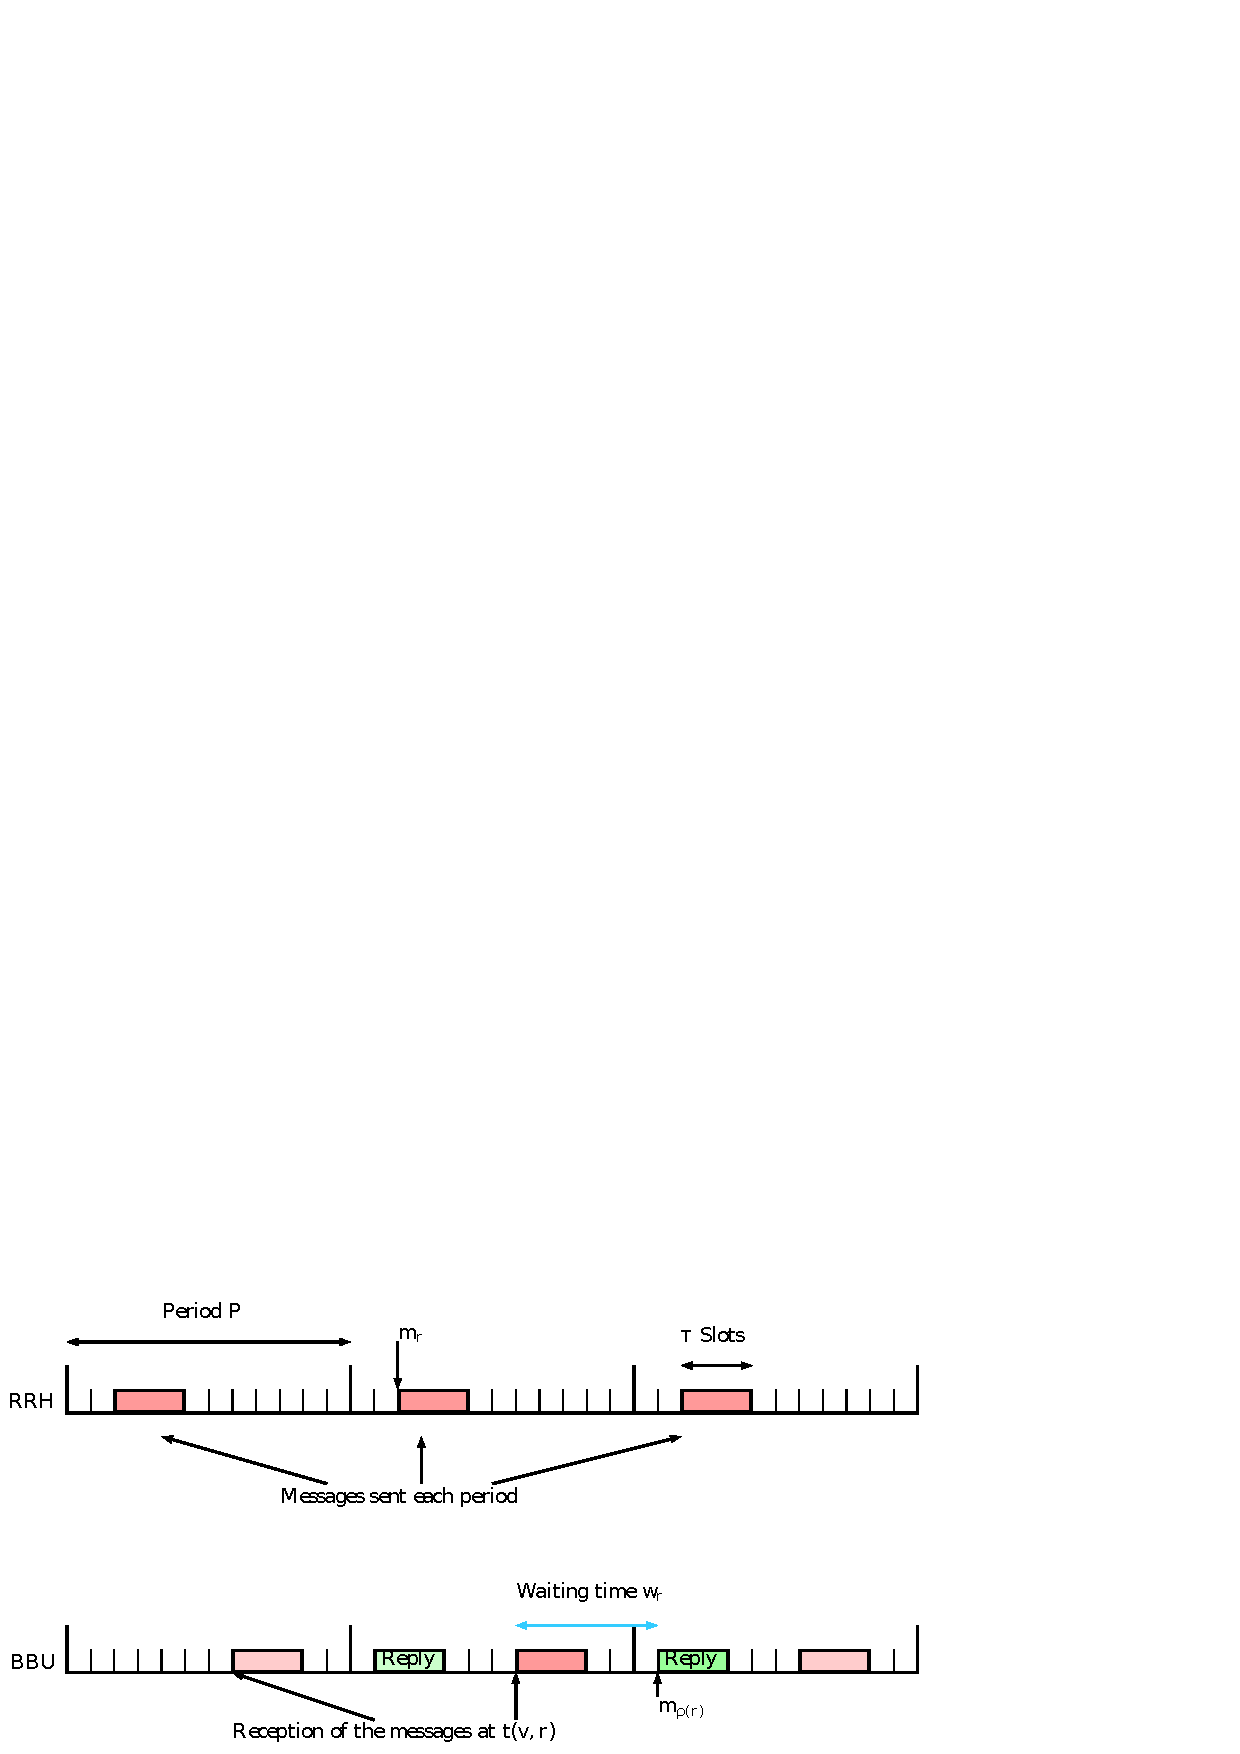
\includegraphics[width = 1cm]{rrh.png}};
   \node[below] at (r2.south) {RRH};
   \node (b1) at (12,0) {\includegraphics[width = 1cm]{bbu.png}};
   \node[below] at (b1.south) {BBU};
   \node (b2) at (12,4) {\includegraphics[width = 1cm]{bbu.png}};
	\node[below] at (b2.south) {BBU};
   \node (s1) at (4,2) {\includegraphics[width = 1cm]{switch.png}};
   \node (s2) at (8,2) {\includegraphics[width = 1cm]{switch.png}};
  
   \node (c) at (6,6) {\includegraphics[width = 1cm]{controller.png}};
   	\node[right] at (c.north east) {Controller};

   	\node (rect) at (6,10) [draw,thick,minimum width=2cm,minimum height=1cm] {Algorithms};

\path (r1) edge [<->]  (s1);
\path (r2) edge [<->]  (s1);
\path (s2) edge [<->]  (s1);
\path (s2) edge [<->]  (b1);
\path (s2) edge [<->]  (b2);
\path (s2) edge [<->]  (c);
\path (s1) edge [<->]  (c);
\path (r1) edge [<->]  (c);
\path (r2) edge [<->]  (c);
\path (b1) edge [<->]  (c);
\path (b2) edge [<->]  (c);
\path (rect) edge [<->]  (c);


\end{tikzpicture}
}



%\end{minipage}

             \caption{An SDN managment allowed by TSN standards.}

           \label{fig:sdncontroller}
            \end{center}
           \end{figure}


\label{sec:TSNqbv}
 TSN is a set of profiles and standards aiming at providing packet forwarding bounded latency. This means that packet latency is within a known interval. This is called « Deterministic Service ». This is rather different from traditional service where no guarantee on latency is given: a packet can be delivered after a very long period of time, depending of the size of the buffers within the network.


 TSN QCC
\section{An experimental prototype}
\label{sec:platform}
- On sait faire des noeuds qui respectent l'organisation

- On sait comment ne pas buffuriser du tout les messages: PALL PAZL

-Voir comment gérer le problème de Dsynch

-parler des reseaux sans aucun buffers intermediaires evoqués dans les chapitres PAZL et PALL
\subsection{Hyper-TSN switch}

An Hyper-TSN switch has been developped. It is composed of a deterministic scheduler, two 10 Gbps ethernet ingress and two 10 Gbps ethernet egress ports. The deterministic scheduler is configured with a timing table. This table is similar to a 802,1 Qbv Gate Control List (GCL). It defines the periodicity of the scheduling and, for each port, the planed date of arrival of the datagrams. At each of these dates the deterministic scheduler sets the switch to transmit data incoming on a specified ingress port.

To perform experiments a generator of deterministic flows has been developed on a Xilinx FPGA board,Zynq-7000 SoC zc706. This generator offsets the dates it sends the frames according to the controls received from the monitoring circuitry.

To perform the experiment the generator is configured to send frames on both egress ports according to the period defined in the timing table. The size of the frames is set to fully load the ethernet links (ie $100\%$ load).

When starting, the monitoring circuitry detects that frames do not arrive at the planed date and sends control commands to the generator. These first frames are lost. Once the generator has rightly offset the dates it sends the frames, nor more offset has been performed during the running 2 hours experiment.

Then $100\%$ of the frames are correctly switched without being corrupted or lost. The switching of each frame from the ingress port to the planed egress port is performed introducing only one clock cycle delay (here 3,87 ns).
